% Chapter 3

\chapter{Understanding the origins of the satellite galaxy distribution in central haloes.} 
\label{Chapter:GalDist}
\lhead{Chapter 3. \emph{Satellite Distributions}} % Write in your own chapter title to set the page header

\section{Background}
%What do we know about the distributions of galaxies
In the \LCDM model of the universe the hierarchical growth of haloes and the resulting dark matter substructure implies that galaxies should be similarly clustered. Satellite galaxies situated in dark matter clusters can therefore be used as tracers of dark matter and used to constrain the cosmological parameters withing a given \LCDM cosmology.
In this chapter we explore the ability of \steel to reproduce satellite distributions over multiple epochs. We also use \steel to test the affect of changing: the dynamical friction timescale, stripping of satellite stellar mass, and star formation rate. By comparing to SDSS we are able to identify the magnitude of each of these affects on the satellite distribution. Understanding the strength of these effects is crucial to understanding the nature of satellites and their mergers with central galaxies.  

\section{Halo Structure and Dynamical Friction}

To understand the evolution of the subhalo/galaxy population we need to isolate which subhalo mass bins from the unevolved subhalo accretion history survive to following epochs. The sum of all the surviving subhaloes (at each epoch) then yields the  unevolved surviving SHMF. 

\subsection{Subhalo Merging Timescale}
\label{sec:Timescale}
 A key parameter used to calculate the unevolved surviving SHMF is the ``observability timescale'' (or survival time) of each  subhalo mass bin $[M_{h,sat}(z),$ $M_{h,sat}(z) + dM_{h,cent}(z)]$ associated to a parent halo mass bin $[M_{h,cent}(z),$ $M_{h,cent}(z) + dM_{h,cent}(z)]$. This timescale is equivalent to the merger timescale $\tau_{merge}$ of a subhalo of mass $M_{h,sat}$ in a parent halo mass $M_{h,cent}$. To calculate $\tau_{merge}$ we use the routines in Equation \ref{eqn:Tmerge} derived from N-body simulations \citep{Boylan-Kolchin2008},

\begin{equation}
\label{eqn:Tmerge}
\tau_{merge} =
(f_{t_{dyn}}\tau_{dyn}) \frac{A(M_{h, cent}/M_{h,sat})^B}{\ln(1+M_{h, cent}/M_{h, sat})} \exp \Big(C\frac{J}{J_c(E)}\Big) \Big( \frac{r_c(E)}{r_{vir}} \Big)^D,
\end{equation}

where A=0.9, B=1.0, C=0.6, D=0.1 \citep{McCavana2012TheMergers}. The factor $\tau_{dyn}$ is given by \citep{Jiang2016StatisticsFunctions},

\begin{equation}
\label{eqn:tdyn}
%t_{dyn} = N \cdot 0.1 \cdot {H(z)}^{-1} 
\tau_{dyn} = 1.628 h^{-1} \mathrm{Gyr} \Big(\frac{\Delta_{vir}(z)}{178}\Big)^{-\frac{1}{2}} \Big(\frac{H(z)}{H_0}\Big)^{-1} \, .
\end{equation}

Our method of considering average halo mass and accretion histories does not permit tracking single orbits and associated orbital energies. We assume instead an average orbit circularity of 0.5 \citep{Khochfar2006OrbitalHalos}, thus reducing the dependence on the angular momentum and radial components, $\frac{J}{J_c(E)}$ and $\frac{r_c(E)}{r_{vir}}$, to a constant. In other words, this approximation is consistent with the approach of taking the average expected orbits of subhaloes at fixed parent halo mass.
The key parameter of our analysis is the factor $f_{t_{dyn}}$ included in Equation \ref{eqn:Tmerge}.
The fudge factor $f_{t_{dyn}}$ takes into account the systematic uncertainties induced by numerical resolution effects in N-body simulations which are unable to resolve the full merging timescales of subhaloes and/or the satellite galaxies they host \citep{vandenBosch2018DisruptionFiction}. The parameter $f_{t_{dyn}}$ increases or decreases the dynamical times of  ``merging'' satellites enabling an exploration of the effect of dynamical time on the final number density distributions of satellite galaxies at any given epoch.

\subsection{Surviving Subhalo Population}
At each redshift we use the unevolved subhalo accretion history and the observability timescale $\tau_{merge}$ to calculate the total observable subhalo population associated with any given parent halo mass bin $[M_{h,cent}(z),$ $M_{h,cent}(z) + dM_{h,cent}(z)]$, i.e. the unevolved surviving SHMF (shown by the dashed lines in Figure \ref{fig:SHMF_clus}). To compute the implied total number densities of unmerged subhaloes with mass $[M_{h,sat}(z),$ $M_{h,sat}(z) + dM_{h,sat}(z)]$ at any redshift of interest we convolve the unevolved surviving SHMF with the HMF,

\begin{equation}
\label{eqn:GSHMF}
N(M_{h, sat}, z) =
\int USSHMF\Bigg(\frac{M_{h, sat}}{M_{h, cent}}\Bigg)HMF(M_{h, cent}, z)dM_{h, cent}.
\end{equation}

Figure \ref{fig:SHMF} shows the total observable subhalo population for different  $f_{t_{dyn}}$ similar to the SHMF in Figure \ref{fig:SHMF_clus}. Furthermore, via appropriate abundance matching algorithms, we can assign corresponding satellite galaxies to the unevolved subhalo accretion history and obtain the distribution of satellites in a given parent halo mass bin $[M_{h,cent}(z),$ $M_{h,cent}(z) + dM_{h,cent}(z)]$ by assuming the satellites follow the same merging timescales as their host subhaloes.

\begin{figure}
	\centering
	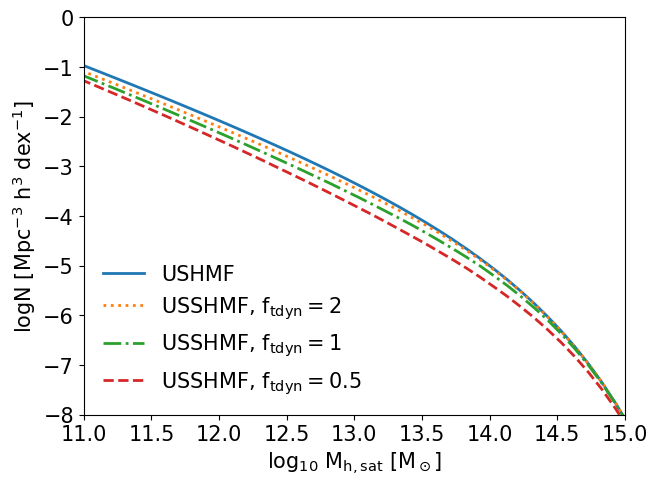
\includegraphics[width = \linewidth]{Figures/Chapter3/SHMF.png}
	\caption{Example of the `total' unevolved SHMF (solid line) and three `total' unevolved surviving SHMF (dotted lines) corresponding to three different $f_{t_{dyn}}$ factors.}
	\label{fig:SHMF}
\end{figure}

\section{Observed Satellite Distributions}

As shown in Equations \ref{eqn:Tmerge} and \ref{eqn:tdyn} the dynamical friction/observibility timescale is dependent on the ratio of halo to sub-halo mass. In Figure \ref{fig:Tdyn_M} in the left hand panel the merging timescales for subhaloes falling into three different central masses at redshift $z=3$ are shown. In each case smaller subhaloes with lower mass ratios have longer merging times, for subhaloes that are significantly under an order of magnitude of mass of the central the merging timescales can extend past $z=0$ and such objects would be present in halo structures today. Associating galaxies to subhaloes we can repeat the exorcise with satellite galaxies similarly it is found that small galaxies in massive haloes are the only galaxies accreted at redshift $z = 1.5$ that one would expect to still be orbiting local galaxies.

\begin{figure}[h]
	\centering
	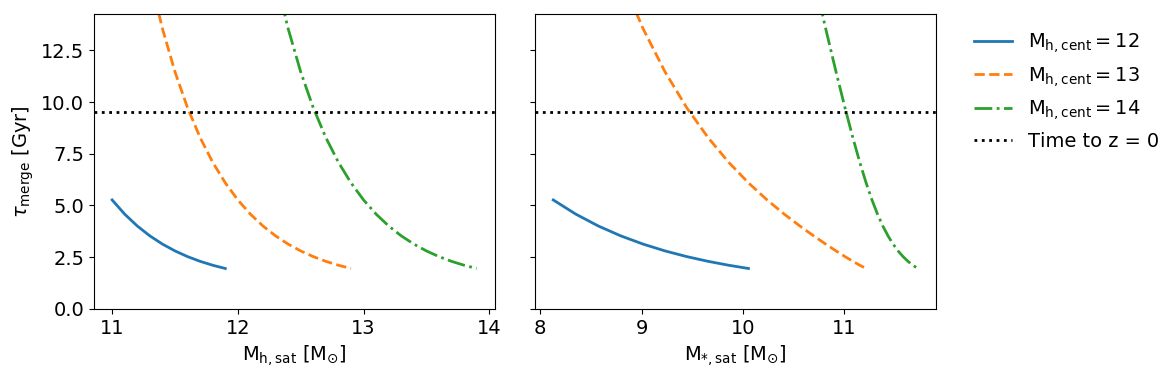
\includegraphics[width = \linewidth]{Figures/Chapter3/Tdyn_M.png}
	\caption{The range of merging timescales for a range of subhalo (left) and satellite (right) masses when accreted at $z = 1.5$ onto three different host masses: $\log$ $M_{h, cen}$ $[M_{\odot}]$ = 12 (blue solid), 13 (orange dashed) and 14 (green dot-dashed). The dotted black line shows the time to redshift $z = 0$, i.e. the minimum amount of time a satellite would need to survive to be observable in the local universe.}
	\label{fig:Tdyn_M}
\end{figure}

In Figure \ref{fig:AccretionTime} the practical affect of increasing the dynamical time is shown. Increasing the dynamical time factor $f_{tdyn}$ to infinity satellites will never merge with the central and thus the right hand panel shows the total buildup of satellites over cosmic time. In the right hand panel with $f_{tdyn} = 1$ we see how the population of satellites still observable at $z=0.1$ is built up over time. As expected from Figure \ref{fig:Tdyn_M} only recently accreted massive satellite galaxies contribute to the observable population where as smaller galaxies will have a wider distribution of accretion times, notably there are no galaxies accreted before redshift $z=2$.

\begin{figure}[h]
	\centering
	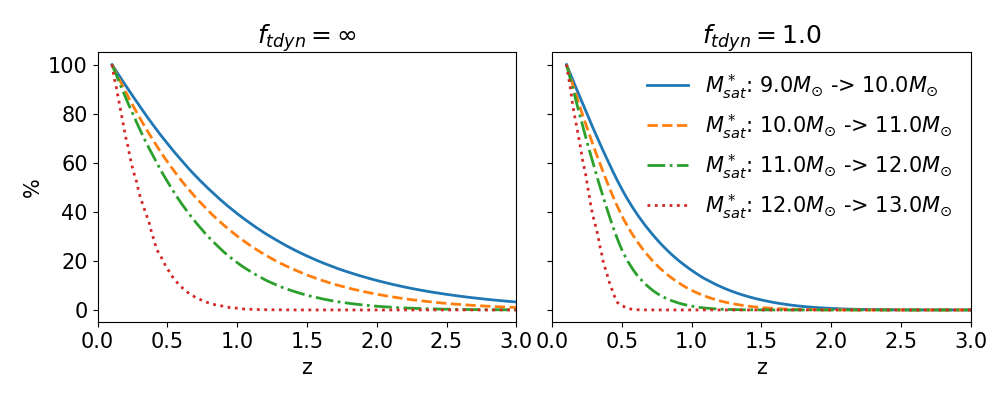
\includegraphics[width = \linewidth]{Figures/Chapter3/AccretedSatellitePercentage.png}
	\caption{We show the percentage of satellites observed at a $z = 0.1$ as a function of their redshift of accretion $z > 0$. It can be seen that massive satellites observed at $z = 0.1$ are accreted more recently than smaller satellites. At $z = 0.5$ less that 50\% of the total satellites observed at $z = 0.1$ have been accreted, and at $z = 0.1$ this falls to less than 20\%. }
	\label{fig:AccretionTime}
\end{figure}

When computing the distribution of satellites as a function of parent halo mass we show both full number densities, as well as fractional distributions to better highlight the ``skewness'' of the predicted distributions with respect to the data. The latter will be simply computed as
\begin{equation}
\label{eqn:FracPlot}
F(dM_h) = \frac{N(>10^x)|_{dM_h}}{N(x)},
\end{equation} 
where $N(>10^{x})$ is the total number (density) of satellites above a threshold stellar mass $x= \log M_{*}$, and the $N(>10^{x})|_{dM_h}$ is the number of these that reside within the halo mass bin $[M_h, M_h+dM_h]$. 

\subsection{Dynamical Friction}
%Show the dynamical friction model and how that actually impacts the distribution.
In this Section we show the prediction of \steel with different merging timescales, $f_{tdyn}$ = $0.5, 1.0, 2.5$, to probe the effects of dynamical time on the satellite population. In Figure \ref{fig:SMF_Tdyn} we find, as expected, that longer dynamical times tend to increase satellite number densities especially towards lower stellar masses. The number densities of higher-mass satellites are more resilient to increase with dynamical time. In fact, when $f_{tdyn}\gtrsim 1$ the number densities of massive satellites become already very close to the theoretical maximum number density when  $f_{t_{dyn}} = \infty$. This trend is also seen in Figure \ref{fig:AccretionTime} the difference between the buildup of high mass satellites between $f_{t_{dyn}} = \infty$ and $f_{t_{dyn}} = 1$ is much less significant than between that of low mass satellites
It follows that massive satellites are on average a recently accreted population. In other words, there are only a few high mass satellites that had enough time to merge when $f_{tdyn}\gtrsim 1$. In contrast, lower mass satellites have not yet reached their theoretical limit, and thus they still have room to increase their number densities with increasing dynamical time.  

Figure \ref{fig:Distrbution_Tdyn} shows how the distribution of satellites, above three stellar mass cuts, as a function of parent halo mass is affected by $f_{tdyn}$. The number density distribution (top row) shows results similar to the satellite SMF where increasing dynamical time increases the number densities. However, there is also an apparent steepening effect for which lower mass host haloes end up containing relatively less satellites with respect to models with longer dynamical times. The fractional plot (bottom row) accentuates this change in the number density distributions shown in the top row: shorter dynamical times shift the peak of the distribution to the right as relatively more satellites are observed in high mass host haloes.

This steepening of the satellite distribution as a function of halo mass, as well as the shift mentioned in Section \ref{subsub:EvoInf} where infinite dynamical times move satellites preferentially to lower halo masses, are both caused by the amount of time satellites survive in their hosts. Massive satellites are far more common in massive hosts, as can be inferred from the SHMF. Therefore, irrespective of the chosen merging timescale, there will always be a high number density of surviving massive satellites in higher mass parent haloes. However, when merging timescales are increased, the lower number densities of massive satellites in moderately-sized haloes are also increased. Given that lower mass parent haloes are more abundant, the reduction of merging timescales tends to shift the peak of the fractional distribution of galaxies to lower mass parents. Otherwise put, the merging timescales in clusters ($ \log_{10} M_{h,cent}$ $[M_{\odot}]$ $> 13.75$) are so long that even a factor five reduction in merger timescale still does not give the satellite galaxies sufficient time to merge with the central galaxy. This effect can be inferred from Figure \ref{fig:Tdyn_M}, where we see steeper gradients for a given subhalo/satellite mass with increasing parent halo mass. Merging is more efficient for the lower mass satellites as can be seen by the steepness of the $f_{t_{dyn}} = 0.5$ model (dashed lines) in the top row of Figure \ref{fig:Distrbution_Tdyn}.

%dynamical distributions

\begin{figure}[h]
	\centering
	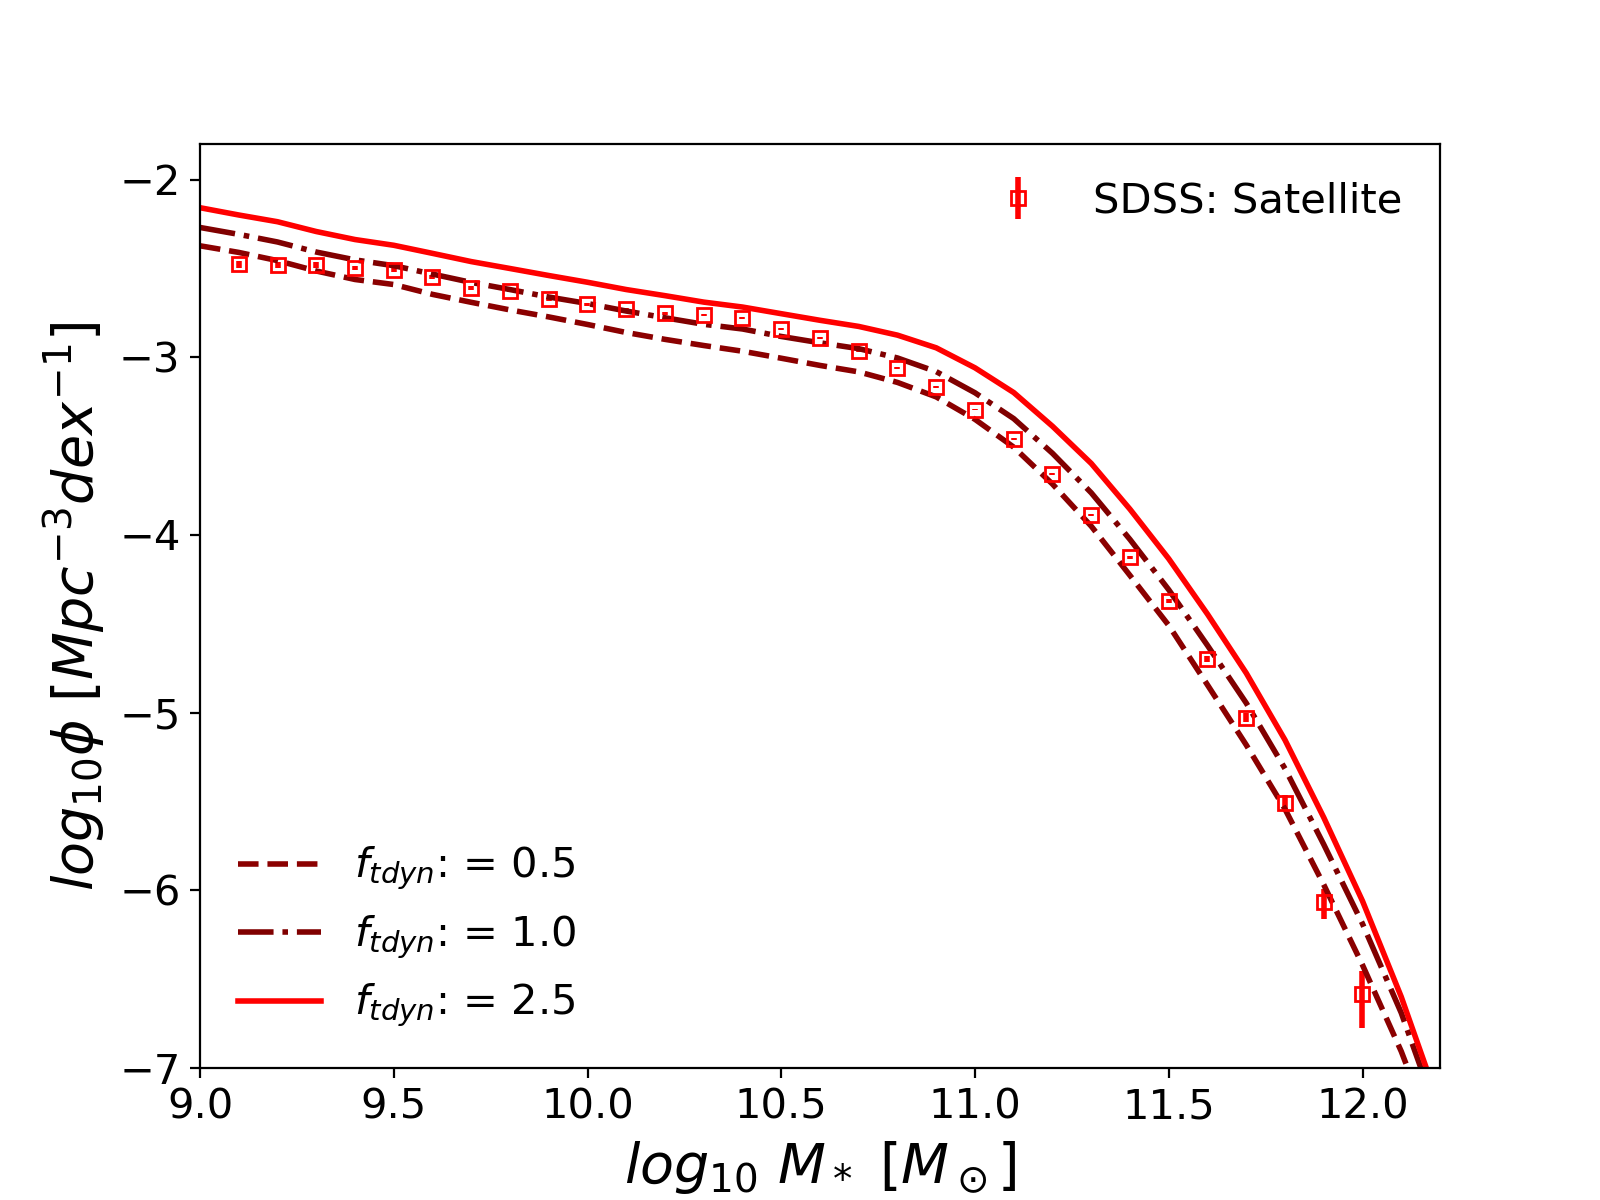
\includegraphics[width = \linewidth]{Figures/Chapter3/Tdyn_SMF.png}
	\caption{Satellite stellar mass functions generated by the model compared to SDSS data (open squares). The solid, dot dashed, and dashed lines show $f_{tdyn} = 0.5, 1.0,$ and $2.5$ respectively.}
	\label{fig:SMF_Tdyn}
\end{figure}

\begin{figure}[h]
	\centering
	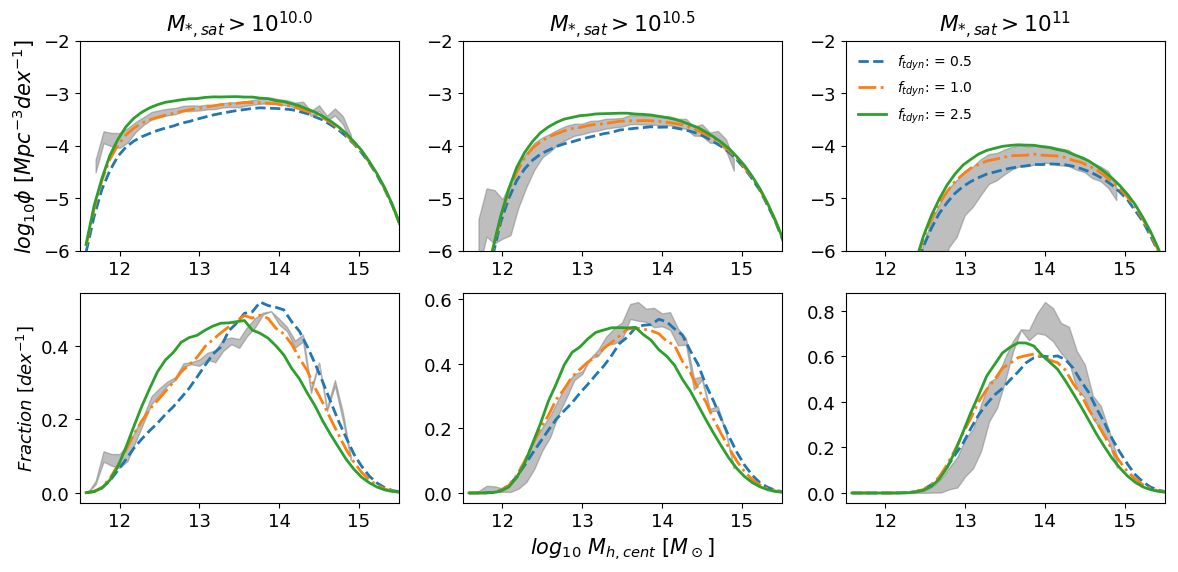
\includegraphics[width = \linewidth]{Figures/Chapter3/Tdyn_Sat_Dist.png}
	\caption{Satellite distributions in parent haloes generated from the model are compared to those observed in SDSS (grey band). Columns from left to right show increasing satellite stellar mass cuts as labelled. The top row shows the number density of satellites expected to be found in each parent halo mass. The bottom row shows the fractional distribution described by Equation \ref{eqn:FracPlot}. The dashed, dot dashed, and solid lines show $f_{tdyn} = 0.5, 1.0,$ and $2.5$ respectively. The width of the grey band corresponds to a 10\% uncertainty in satellite stellar masses.}
	\label{fig:Sat_Dist_Tdyn}
\end{figure}

The least-square residuals to the SMF, number density distribution and fractional distributions are given in Table \ref{tab:bestfit}. There is no model that simultaneously fully matches all the observations in all mass ranges. The trend in both the number density distribution and the fractional distribution is that slightly longer dynamical times ($f_{tdyn}  = 1.2$) are favored by the less massive satellites. Longer dynamical timescales better match the halo mass distributions (number density distribution/fractional distributions) for lower mass satellites, and vice versa for higher mass satellites with $\log M_{*}/M_{\odot} >11$. Nevertheless, the simple combination of abundance matching and dynamical merging timescales as suggested by pure N-body simulations ($f_{t_{dyn}} = 1.0$) tends to provide overall good agreement to both the satellite SMF and the satellite distributions, without the need to invoke additional physics in the (late) evolution of satellite galaxies after infall.

\begin{table*}
\centering
\caption{We show the sum of the squared residuals between the SDSS and our model. The satellite SMF is calculated between 9.1 and 12.0 $M_{*}$. The SDF fit is calculated between 12 and 14.9 $M_h$ for the \textgreater10 and\textgreater10.5 plots, and between 12.5 and 14.9 $M_h$ for \textgreater11. The Fractional plot fit is calculated between 11.6 and 14.9 $M_h$.}
\label{tab:bestfit}
\begin{tabular}{c|c|ccc|ccc}
$f_{t_{dyn}}$   & SSMF   (Fig \ref{fig:SMF_Tdyn})               & \multicolumn{3}{c}{SDF  } \vline & \multicolumn{3}{c}{Fractional Distribution } \\
   &   (Fig \ref{fig:SMF_Tdyn})               & \multicolumn{3}{c}{ (Top Row Fig \ref{fig:Sat_Dist_Tdyn}) } \vline & \multicolumn{3}{c}{ (Bottom Row Fig \ref{fig:Sat_Dist_Tdyn})} \\ \hline
            \multicolumn{1}{l}{} \vline & \multicolumn{1}{l}{} \vline & \multicolumn{1}{l}{\textgreater{}10} & \multicolumn{1}{l}{\textgreater{}10.5} & \multicolumn{1}{l}{\textgreater{}11} \vline & \multicolumn{1}{l}{\textgreater{}10} & \multicolumn{1}{l}{\textgreater{}10.5} & \multicolumn{1}{l}{\textgreater{}11} \\ \hline
0.5    & 0.022   & 0.19  & 0.55    & 0.073    & 0.0042 & 0.0047 & 0.0078  \\
0.8    & 0.025   & 0.13  & 0.51    & 0.089    & 0.0020 & 0.0017 & 0.0054  \\
1.0    & 0.034   & 0.12  & 0.56    & 0.10     & 0.0015 & 0.0011 & 0.0050  \\
1.2    & 0.043   & 0.12  & 0.53    & 0.11     & 0.0015 & 0.00094& 0.0046  \\
1.5    & 0.054   & 0.12  & 0.52    & 0.13     & 0.0017 & 0.0010 & 0.0045                              
\end{tabular}
\end{table*}

%show stripping/SF routines and their effects
\subsection{Evolutionary models}

The prior section makes an implicit assumption that satellites do not evolve after infall. In this section we apply several evolutionary affects to the satellites assuming they have the same properties as centrals at infall then evolve in response to their environment. 


\subsubsection{Star Formation Rates}
We use the star formation rate (SFR) parameterization from \citet{Lee2015A1.3} with parameters\footnote{These parameters are derived by fitting data from ZFORGE in combination with far-IR imaging from \textit{Spitzer} and \textit{Herschel} in the range $0.5<z<4$. In this work we extrapolate their fits down to $z = 0$, as this is consistent with the SFR measured by  \cite{Salim2007UVUniverse} at lower redshifts.} from \cite{Tomczak2016THE4} where $s_0$ and $M_0$ have units $log(M_{\odot})$ and $M_{\odot}$ respectively,

\begin{equation}
\begin{split}
\label{eqn:SFR}
\log[\psi(z, M_*)] &= s_0(z) - \log \Big[ 1 + \Big(\frac{M_*}{M_0(z)}\Big)^{-\alpha(z)}\Big] \\
s_0(z) &= 0.195 + 1.157z - 0.143(z^2) \\
\log[M_0(z)] &= 9.244 + 0.753z - 0.090(z^2) \\
\alpha(z) &= 1.118.
\end{split}
\end{equation}

As discussed continuity-equation approaches are more suited to modelling due to the inconsistencies in growth of the SMF and the observed SFR \citep{Leja2015ReconcilingFunction}. We have refitted the parameters in Equation \ref{eqn:SFR} to match the SFR distributions expected from self-consistently growing the stellar mass functions used as input in our models. The fit to the resulting SFRs is given by

\begin{equation}
\begin{split}
\label{eqn:SFR_CE}
\log(\psi(z, M_*)) &= s_0(z) - \log \Big[ 1 + \Big(\frac{M_*}{M_0(z)}\Big)^{-\alpha(z)}\Big] \\
s_0(z) &= 0.6 + 1.22z - 0.2(z^2) \\
\log(M_0(z)) &= 10.3 + 0.753z - 0.15(z^2) \\
\alpha(z) &= 1.3 - 0.1z.
\end{split}
\end{equation}
In all cases the SFR is included in our models with a log-normal scatter of 0.3 dex \citep{Leja2015ReconcilingFunction}.


In what follows we explore the two star formation rate models with the quenching model described in Sections \ref{sec:SFR} and \ref{sec:QuenchingModels}. 


The first, purely observationally-based, star formation rate model strictly follows the SFR parametrization by \citet[][T16 hereafter]{Tomczak2016THE4}, given in Equation \ref{eqn:SFR}. The second star formation rate model (which we label as ``CE'') is instead based on a continuity equation approach similar to \cite{Leja2015ReconcilingFunction}. In essence, the latter is based on first assuming number conservation of galaxies, and then deriving the implied star formation rates as a function of stellar mass from the time growth in any stellar mass bin implied by the redshift evolution of the stellar mass function (corrected for gas loss from dying stars assumed to be an average of 40\%). The novelty in the latter model with respect to previous work is that we do not tune the resulting star formation rate on the total but rather only on the stellar mass function of \textit{central} galaxies, which is in turn iteratively constrained by matching the local stellar mass function of SDSS centrals. This has the main effect of lowering the implied average star formation rate at fixed stellar mass at any given epoch (see Equations \ref{eqn:SFR} and \ref{eqn:SFR_CE}).

\begin{figure}
	\centering
	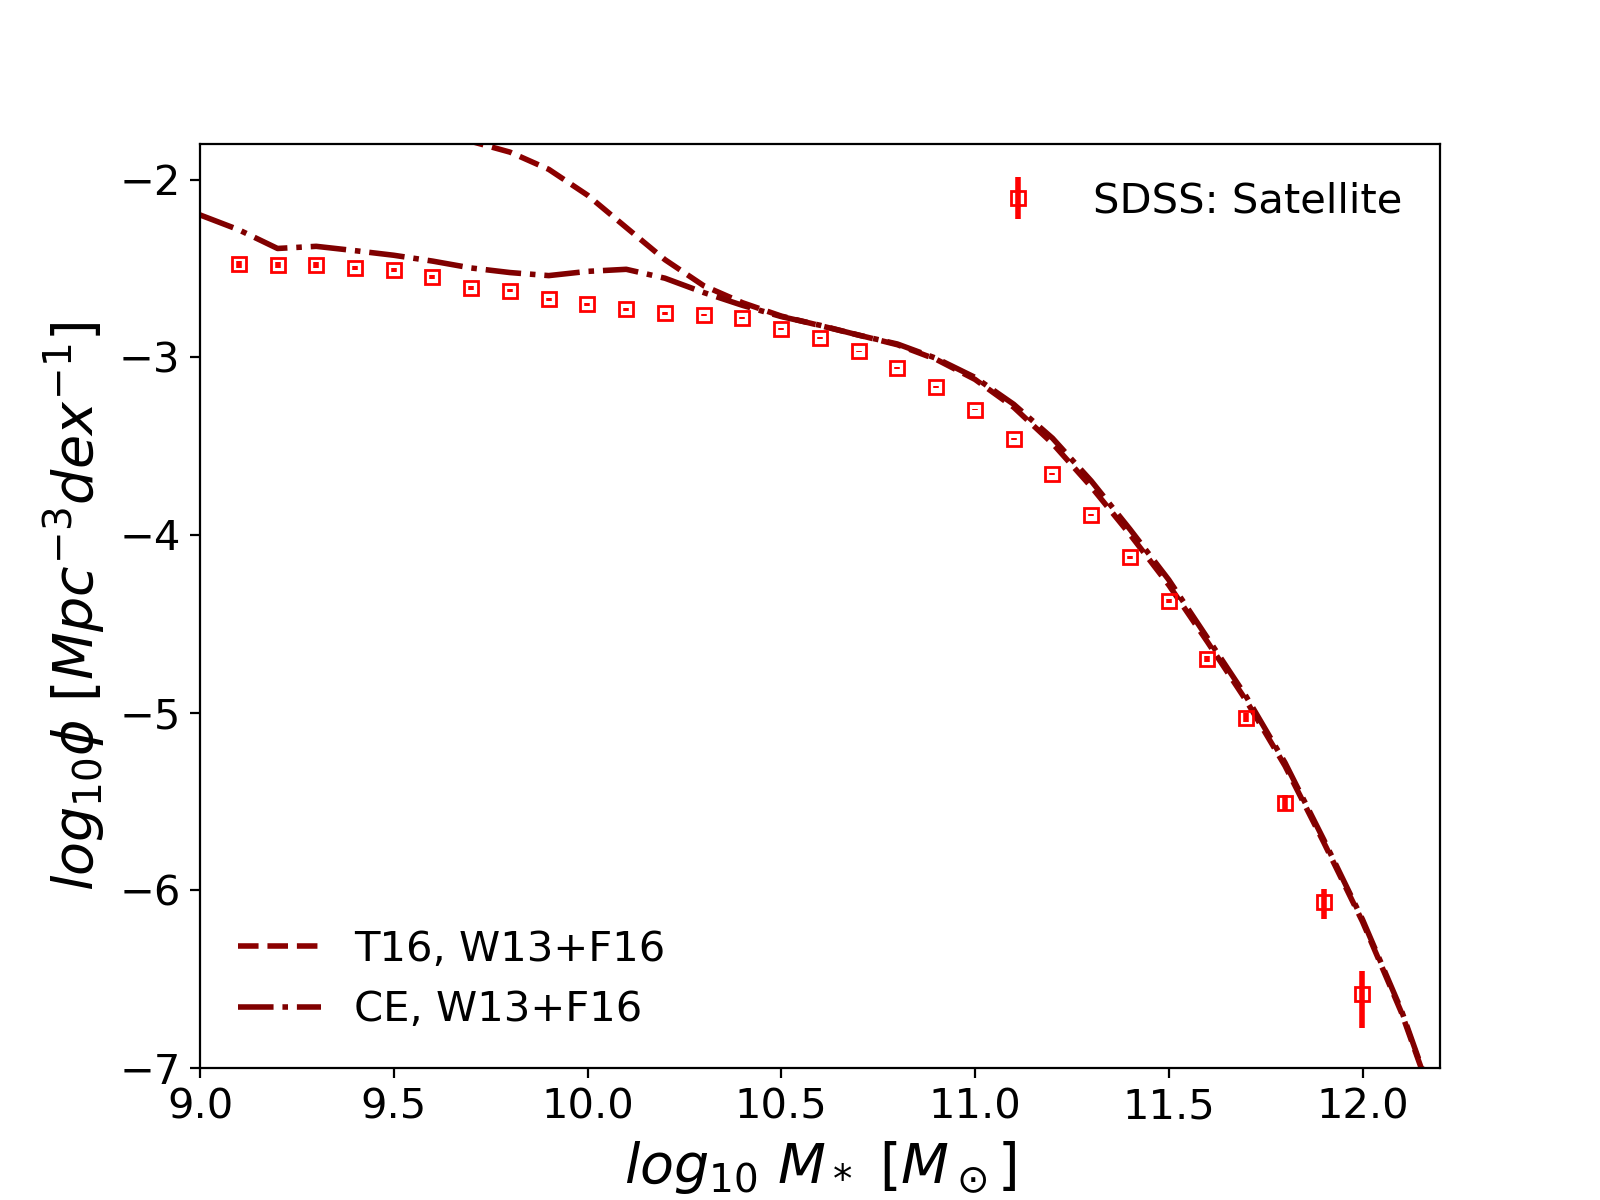
\includegraphics[width = \linewidth]{Fig9.png}
	\caption{Satellite stellar mass functions generated from the model using both the \citet{Tomczak2016THE4} (dashed) and continuity (dot dashed) star formation rates compared to the SDSS satellite stellar mass function (open squares).}
	\label{fig:SMF_SF_Q}
\end{figure}

We compare the satellite SMFs produced by the two star formation+quenching models addressed above to our SDSS stellar mass function of satellites in Figure \ref{fig:SMF_SF_Q}. It is apparent that using the observed SFR by T16 (dashed line), even inclusive of the best recipes for quenching, still substantially overproduces the number density of galaxies below $M_* \lesssim 3\times 10^{10}\, M_{\odot}$. This is a well-known problem affecting the full (dominated by central) galaxy population \citep[e.g.,][]{Leja2015ReconcilingFunction}: the integrated (observed) SFR is not consistent with the moderate growth over time of the SMF causing an overproduction of galaxies becoming gradually more severe at lower stellar masses. Our results point to a similar problem affecting the satellite population, on the assumption that the latter at infall share the same SFR distribution as a typical central galaxy of the same stellar mass.





\begin{figure}
	\centering
	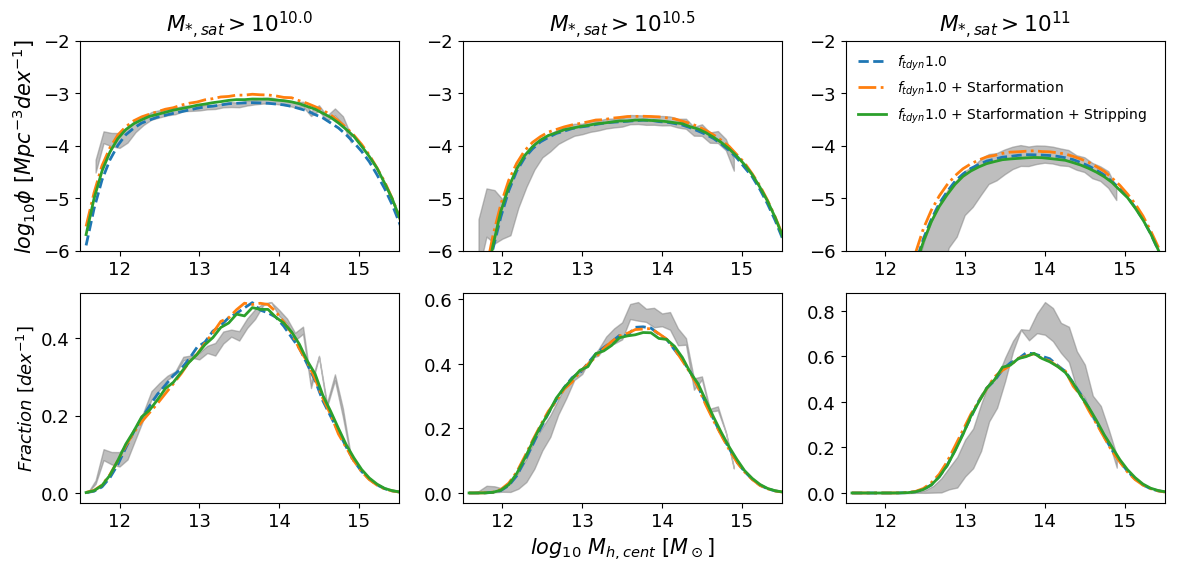
\includegraphics[width = \linewidth]{Figures/Chapter3/Sat_Dist_SF_Strip.png}
	\caption{Satellite distributions in parent haloes generated from the model are compared to those observed in SDSS (grey band). Columns from left to right show increasing satellite stellar mass cuts as labelled. The top row shows the number density of satellites expected to be found in each parent halo mass. The bottom row shows the fractional distribution described by Equation \ref{eqn:FracPlot}. The models shown all have $f_{tdyn} = 1.0$ and are the reference 'frozen model' (dashed line), starformation only (dot dashed line) and starformation and stripping (solid line). The width of the grey band corresponds to a 10\% uncertainty in satellite stellar masses.}
	\label{fig:Sat_Dist_SF_Strip}
\end{figure}



\section{Multi-Epoch Distributions of Satellite Galaxies}

\begin{figure}[h]
	\centering
	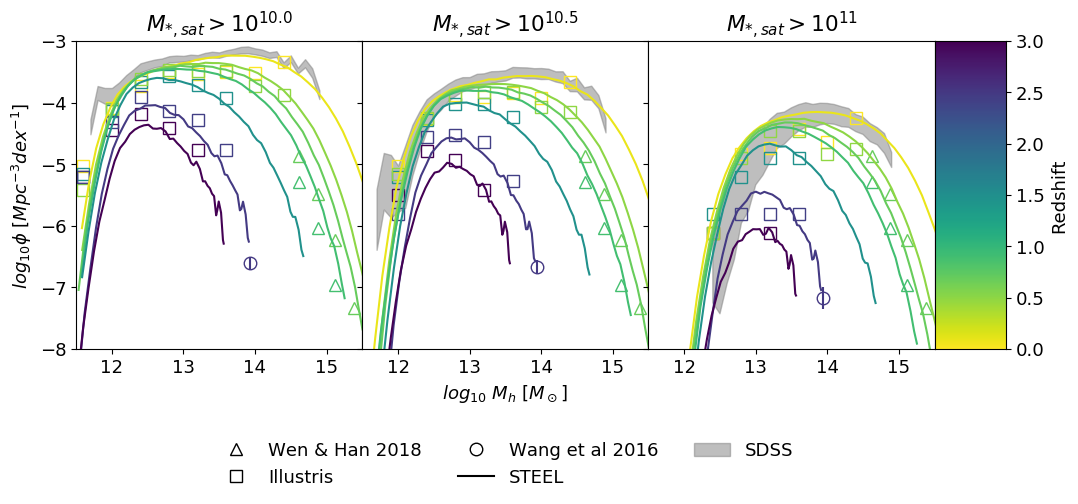
\includegraphics[width = \linewidth]{Figures/Chapter3/HighzClusters.png}
    \caption{The number-density distribution of satellites per parent halo mass predicted from \textsc{steel}, using the PyMorph SMHM relation, at multiple redshift epochs (solid lines). The grey band is the data from SDSS at redshift $z=0.1$. Also included are the high redshift cluster data from \citet{Wang2016DiscoveryZ=2.506} (circles) and \citet{Wen2018ARedshifts} (triangles). I also compare to the outputs from the Illustris simulation using the TNG100 data (crosses). Each data point and line are given a colour associated to their redshift (the bar on the right provides the color coding key).}
	\label{fig:Sat_Dist_High_z}
\end{figure}